\section{Process Discovery}
\subsection{Alpha Miner}
\subsubsection{Exercise 1}
Given the following event log:
\[L_1 = [\langle a,b,c,d \rangle^3, \langle a,c,b,d \rangle^2, \langle a,e,d \rangle^1]\]
build the process model using the Alpha Miner algorithm.
\paragraph{Solution}
\begin{enumerate}
    \item 
\end{enumerate}

\subsubsection{Exercise 2}
Given the following event log:
\[L = \left[ \langle a,b,c,d,e,f,b,d,c,e,g \rangle, \langle a,b,d,c,e,g \rangle^2, \langle a,b,c,d,e,f,b,c,d,e,f,b,d,c,e,g \rangle\right]\]
Use the Alpha Miner algorithm to discover a Petri net from the event log.
\paragraph{Solution:}
\begin{enumerate}
    \item First, we need to compute the footprint matrix:
    \begin{table}[H]
    \centering
    \begin{tabular}{c|ccccccc}
        & A & B & C & D & E & F & G \\
        \hline
        A & $\#$ & $\rightarrow$ & $\#$ & $\#$ & $\#$ & $\#$ & $\#$ \\
        B &  & $\#$ & $\rightarrow$ & $\rightarrow$ & $\#$ & $\leftarrow$ & $\#$ \\
        C &  &  & $\#$ & $||$ & $\rightarrow$ & $\#$ & $\#$ \\
        D &  &  &  & $\#$ & $\rightarrow$ & $\#$ & $\#$ \\
        E &  &  &  &  & $\#$ & $\rightarrow$ & $\rightarrow$ \\
        F &  &  &  &  &  & $\#$ & $\#$ \\
        G &  &  &  &  &  &  & $\#$ \\
    \end{tabular}
    \caption{Footprint Matrix for the Event Log \(L\)}
\end{table}
    \item Next, we identify the sets of all transitions $T_L$, the set of start activities $T_I$ and the set of end activities $T_O$:
    \begin{itemize}
        \item $T_L = \{a,b,c,d,e,f,g\}$
        \item $T_I = \{a\}$
        \item $T_O = \{g\}$
    \end{itemize}
    \item Then, we identify the pairs of sets of transitions that satisfy the Alpha Miner conditions.
    To find the first pairs, we look for causality relations in the footprint matrix:
    \[\{
        (\{a\}, \{b\}),\ 
        (\{b\}, \{c\}),\ 
        (\{b\}, \{d\}),\ 
        (\{f\}, \{b\}),\ 
        (\{c\}, \{e\}),\
        (\{d\}, \{e\}),\
        (\{e\}, \{f\}),
        (\{e\}, \{g\})
    \}
    \]
    \item We can then group these pairs into maximal sets:
    \[\{
        (\{a,f\}, \{b\}),\ 
        (\{e\}, \{f,g\}),\
    \}
    \]
    And we can remove the non-maximal sets that composed them:
    \[\{
        (\{a\}, \{b\}),\
        (\{f\}, \{b\}),\
        (\{e\}, \{f\}),\
        (\{e\}, \{g\})
    \}
    \]
    \item Finally, we can construct the Workflow net, using one place for each of the identified pairs, and connecting them according to the causality relations:
    \begin{figure}[H]
        \centering
        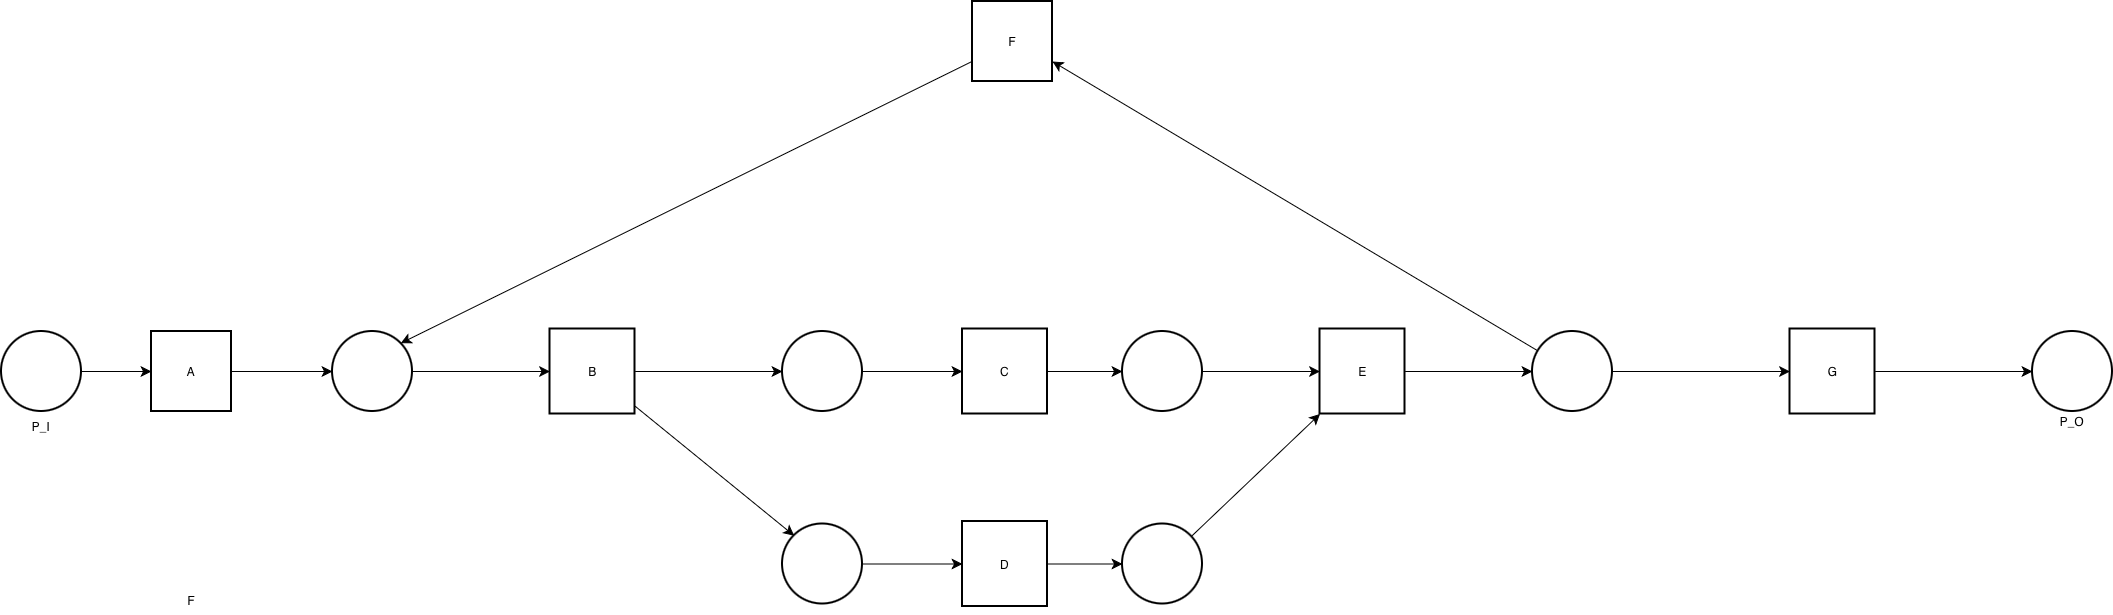
\includegraphics[width=0.7\textwidth]{../images/exercises/alpha_miner.png}
        \caption{Petri Net Discovered using the Alpha Miner}
    \end{figure}
\end{enumerate}
\subsubsection{Exercise 3}
Given the following event log:
\[L_4 = [\langle a,c,d \rangle^{45}, \langle b,c,d \rangle^{42}, \langle a,c,e \rangle^{38}, \langle b,c,e \rangle^{22}]\]
build the process model using the Alpha Miner algorithm.
\paragraph{Solution}
\begin{enumerate}
    \item 
\end{enumerate}

\subsubsection{Exercise 4}
Consider the following event log:
\[L = [\langle a,b,d \rangle^{100}, \langle a,c,b,d \rangle^{80}, \langle a,b,c,d \rangle^{2}, \langle a,c,d \rangle^{40}, \langle a,d \rangle^{1}]\]
Use the Alpha Miner algorithm to discover a Petri net from the event log.
\paragraph{Solution:}

\subsection{Heuristic Miner}
\subsubsection{Exercise 1}
Given the following event log:
\[L = [\langle a,e \rangle^5, \langle a,b,c,e \rangle^{10}, \langle a,c,b,e \rangle^{10}, \langle a,b,e \rangle^{1}, \langle a,c,e \rangle^{1},\]
\[
\langle a,d,e \rangle^{10}, \langle a,d,d,e \rangle^{2}, \langle a,d,d,d,e \rangle^{1}]
\]
use the Heuristic Miner algorithm to discover a process model from the event log, with a threshold of 0.7:
\paragraph{Solution:}
\begin{enumerate}
    \item First, we need to compute the frequency matrix:
    \begin{table}[H]
    \centering
    \begin{tabular}{c|cccccccc}
        & A & B & C & D & E \\
        \hline
        A & 0 & 11 & 11 & 13 & 5 \\
        B & 0 & 0 & 10 & 0 & 11 \\
        C & 0 & 10 & 0 & 0 & 11 \\
        D & 0 & 0 & 0 & 4 & 13 \\
        E & 0 & 0 & 0 & 0 & 0 \\
    \end{tabular}
    \caption{Frequency Matrix for the Event Log \(L\)}
    \end{table}
    Each cell \((x,y)\) contains the number of times activity \(x\) is directly followed by activity \(y\) in the event log.
    \item Next, we compute the dependency matrix, by applying the dependency measure formula to each pair of activities.
    Remember that the dependency measure is defined as:
    \[
    \begin{cases}
        \frac{|x\rightarrow y| - |y\rightarrow x|}{|x\rightarrow y| + |y\rightarrow x| + 1} & \text{if } x \neq y \\
        \frac{|x\rightarrow x|}{|x\rightarrow x| + 1} & \text{otherwise}
    \end{cases}
    \]
    Note that:
    \begin{itemize}
        \item Along the diagonal, we apply the second case of the formula;
        \item We can compute the upper triangle of the matrix, the lower triangle can be derived from it by simply swapping signs.
    \end{itemize}
    \begin{table}[H]
    \centering
    \begin{tabular}{c|cccccccc}
        & A & B & C & D & E \\
        \hline
        A & 0 & $\frac{11}{12}$ & $\frac{11}{12}$ & $\frac{13}{14}$ & $\frac{5}{6}$ \\
        B &  & 0 & $\frac{10 - 10}{21}$ & 0 & $\frac{11}{12}$ \\
        C &  &  & 0 & 0 & $\frac{11}{12}$ \\
        D &  &  &  & $\frac{4}{5}$ & $\frac{13}{14}$ \\
        E &  &  &  &  & 0 \\
    \end{tabular}
    \caption{Dependency Matrix for the Event Log \(L\)}
    \end{table}
    \item We can then build the dependecy graph, using the given threshold.
    We create a node for each activity in the log, and add the directed edges for each pair of activities whose dependency measure is above the threshold:
    \begin{figure}[H]
        \centering
        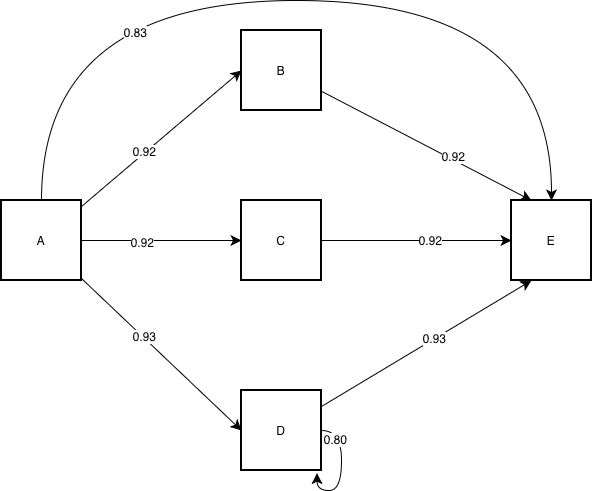
\includegraphics[width=0.7\textwidth]{../images/exercises/heuristic_miner_1.png}
        \caption{Dependency Graph for the Event Log \(L\)}
    \end{figure}
\end{enumerate}
\subsubsection{Exercise 2}
Given the following event log:
\[L_2 = \left[ \langle a,b,d,e \rangle^{80}, \langle a,d,b,e \rangle^{30}, \langle a,e \rangle^{2}, \langle a,b,c,d,e \rangle^{10} \right] \]
use the Heuristic Miner algorithm to discover the dependency matrix from the event log and build the dependency graph with a threshold of 0.9.

\subsubsection{Exercise 3}
Given the following event log:
\[L_3 = \left[ \langle a,b,d \rangle^{100}, \langle a,c,b,d \rangle^{80}, \langle a,b,c,d \rangle^{2}, \langle a,c,d \rangle^{40}, \langle a,d \rangle^{1} \right] \]
Compute:
\begin{itemize}
    \item The frequency matrix;
    \item The dependency matrix;
    \item The dependency graph with a threshold of 0.9 and a threshold for direct succession of 1.
\end{itemize}

\subsection{Region Based Miner}
\subsubsection{Exercise 1}
Construct a transition system applying the \textit{past with multiset abstraction} for the given log:
\[L = [\langle a,c,b,d \rangle, \langle a,b,c,d \rangle, \langle b,a,c,d \rangle]\]
\paragraph{Solution:}
\begin{enumerate}
    \item We create a starting state \(q_0\) with an empty multiset;
    \item We replay each trace in the log, updating the multiset and creating new states as needed. For instance, considering the first trace \(\langle a,c,b,d \rangle\):
    \begin{itemize}
        \item For the event \(a\), we add a transition from \(q_0\) to a new state \(q_1\) with multiset \(\{a\}\);
        \item For the event \(c\), we add a transition from \(q_1\) to \(q_2\) with multiset \(\{a,c\}\);
        \item For the event \(b\), we add a transition from \(q_2\) to \(q_3\) with multiset \(\{a,b,c\}\);
        \item \dots
    \end{itemize}
    Continuing this process for all traces, we obtain the following transition system:
    \begin{figure}[H]
        \centering
        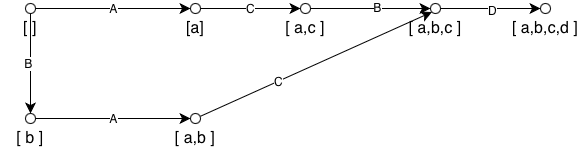
\includegraphics[width=0.7\textwidth]{../images/exercises/region_miner_1.png}
        \caption{Transition System using Past with Multiset Abstraction}
    \end{figure}
\end{enumerate}
\subsubsection{Exercise 2}
Given the previous transition system, compute the resulting Petri net:
\paragraph{Solution:}
\begin{enumerate}
    \item We identify the minimal, non-trivial regions in the transition system. In this case, we have:
    \begin{figure}[H]
        \centering
        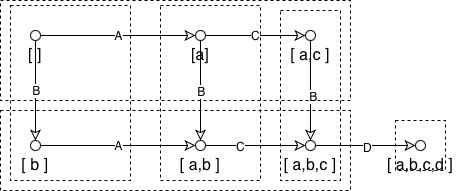
\includegraphics[width=0.7\textwidth]{../images/exercises/region_miner_2.png}
        \caption{Identified Regions from the Transition System}
    \end{figure}
    \item We then create a place for each region. 
    All the transition entering a region will have an arc to the corresponding place, and all transitions leaving the region will have an arc from the place.
    This results in the following Petri net:
    \begin{figure}[H][H]
        \centering
        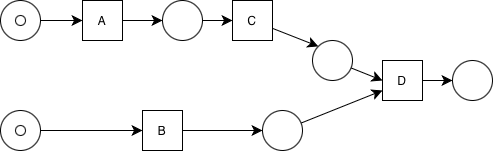
\includegraphics[width=0.7\textwidth]{../images/exercises/region_miner_2-1.png}
        \caption{Petri Net Derived from the Transition System}
    \end{figure}
\end{enumerate}
\subsubsection{Exercise 3}
Given the following event log:
\[L = [\langle a,b,c,d \rangle^3, \langle a,c,b,d \rangle^2, \langle a,e,d \rangle^1]\] 
build the process model using the Region Based Miner algorithm with \textit{past with set abstraction}.
\paragraph{Solution:}

\subsubsection{Exercise 4}
Given the following event log:
\[L = [\langle a,b,d \rangle^{100}, \langle a,c,b,d \rangle^{80}, \langle a,b,c,d \rangle^{2}, \langle a,c,d \rangle^{40}, \langle a,d \rangle^{1}]\]
Use the Region Based Miner algorithm with \textit{past with set abstraction} to discover a Petri Net:

\subsection{Inductive Miner}
\subsubsection{Exercise 1}
Given the following event log:
\[L = [\langle a,b,c,d \rangle^3,
    \langle a,c,b,d \rangle^4,
    \langle a,b,c,e,f,b,c,d \rangle^2,
    \langle a,c,b,e,f,b,c,d \rangle^2,\]
\[
    \langle a,b,c,e,f,c,b,d \rangle,
    \langle a,c,b,e,f,b,c,e,f,c,b,d \rangle 
\]
use the Inductive Miner algorithm to discover a process model from the event log.
\paragraph{Solution:}

\subsubsection{Exercise 2}
Given the following event log:
\[L = [\langle a,c,d \rangle^{45}, \langle b,c,d \rangle^{42}, \langle a,c,e \rangle^{38}, \langle b,c,e \rangle^{22}]\]
use the Inductive Miner algorithm to discover a process model from the event log.

\subsubsection{Exercise 3}
Given the following event log:
\[L = [\langle a,b,d \rangle^{100}, \langle a,c,b,d \rangle^{80}, \langle a,b,c,d \rangle^{2}, \langle a,c,d \rangle^{40}, \langle a,d \rangle^{1}]\]
use the Inductive Miner algorithm to discover a process model from the event log.